\subsection{Posterior Sampling for Bayesian Optimization}
\label{sec:bayesopt_results}

The second application of CIQ we explore is GP posterior sampling in the context of Bayesian optimization \citep[e.g.][]{snoek2012practical}.
Many acquisition functions require drawing samples from GP posteriors \citep[e.g.][]{frazier2009knowledge,hernandez2014predictive,wang2017max}.
One canonical example is {\bf Thompson Sampling} \cite{thompson1933likelihood}, which trades off exploitation of existing minima for exploration of new potential minima.
Thompson sampling simply chooses $\bx_N$ as the minimizer of a sample drawn from the posterior.
Let $\bXtest = [ \bxtest_1, \ldots, \bxtest_T ]$ be a \emph{candidate set} of possible acquisition points.
To choose the candidate point $\widetilde \bx$, Thompson sampling computes
%
\begin{equation}
  \widetilde \bx = \argmin_{i} \left( \bmeantest(\bXtest) + {\Covtest(\bXtest)}^{\frac 1 2} \bepsilon \right),
  \quad
  \bepsilon \sim \normaldist{\bzero}{\bI}.
  \label{eqn:thompson_sample}
\end{equation}
%
where $\bmeantest(\bXtest)$ and $\Covtest(\bXtest)$ are the posterior mean and covariance of the GP applied at the candidate set.
Larger candidate sets (i.e. larger values of $T$) more densely cover the search space, which naturally should result in better acquisition points.
It is therefore beneficial to choose the largest value of $T$ that is computationally feasible.
Using Cholesky to compute \cref{eqn:thompson_sample} incurs a $\bigo{T^3}$ cost which severely limits the size of $T$.
On the other hand, CIQ only requires $\bigo{T^2}$ computation.
Using partitioned MVM methods presented in the next chapter, we can reduce the CIQ memory requirement to $\bigo{T}$ (see \cref{sec:largeexact_method}).

\begin{figure}[t!]
  \centering
  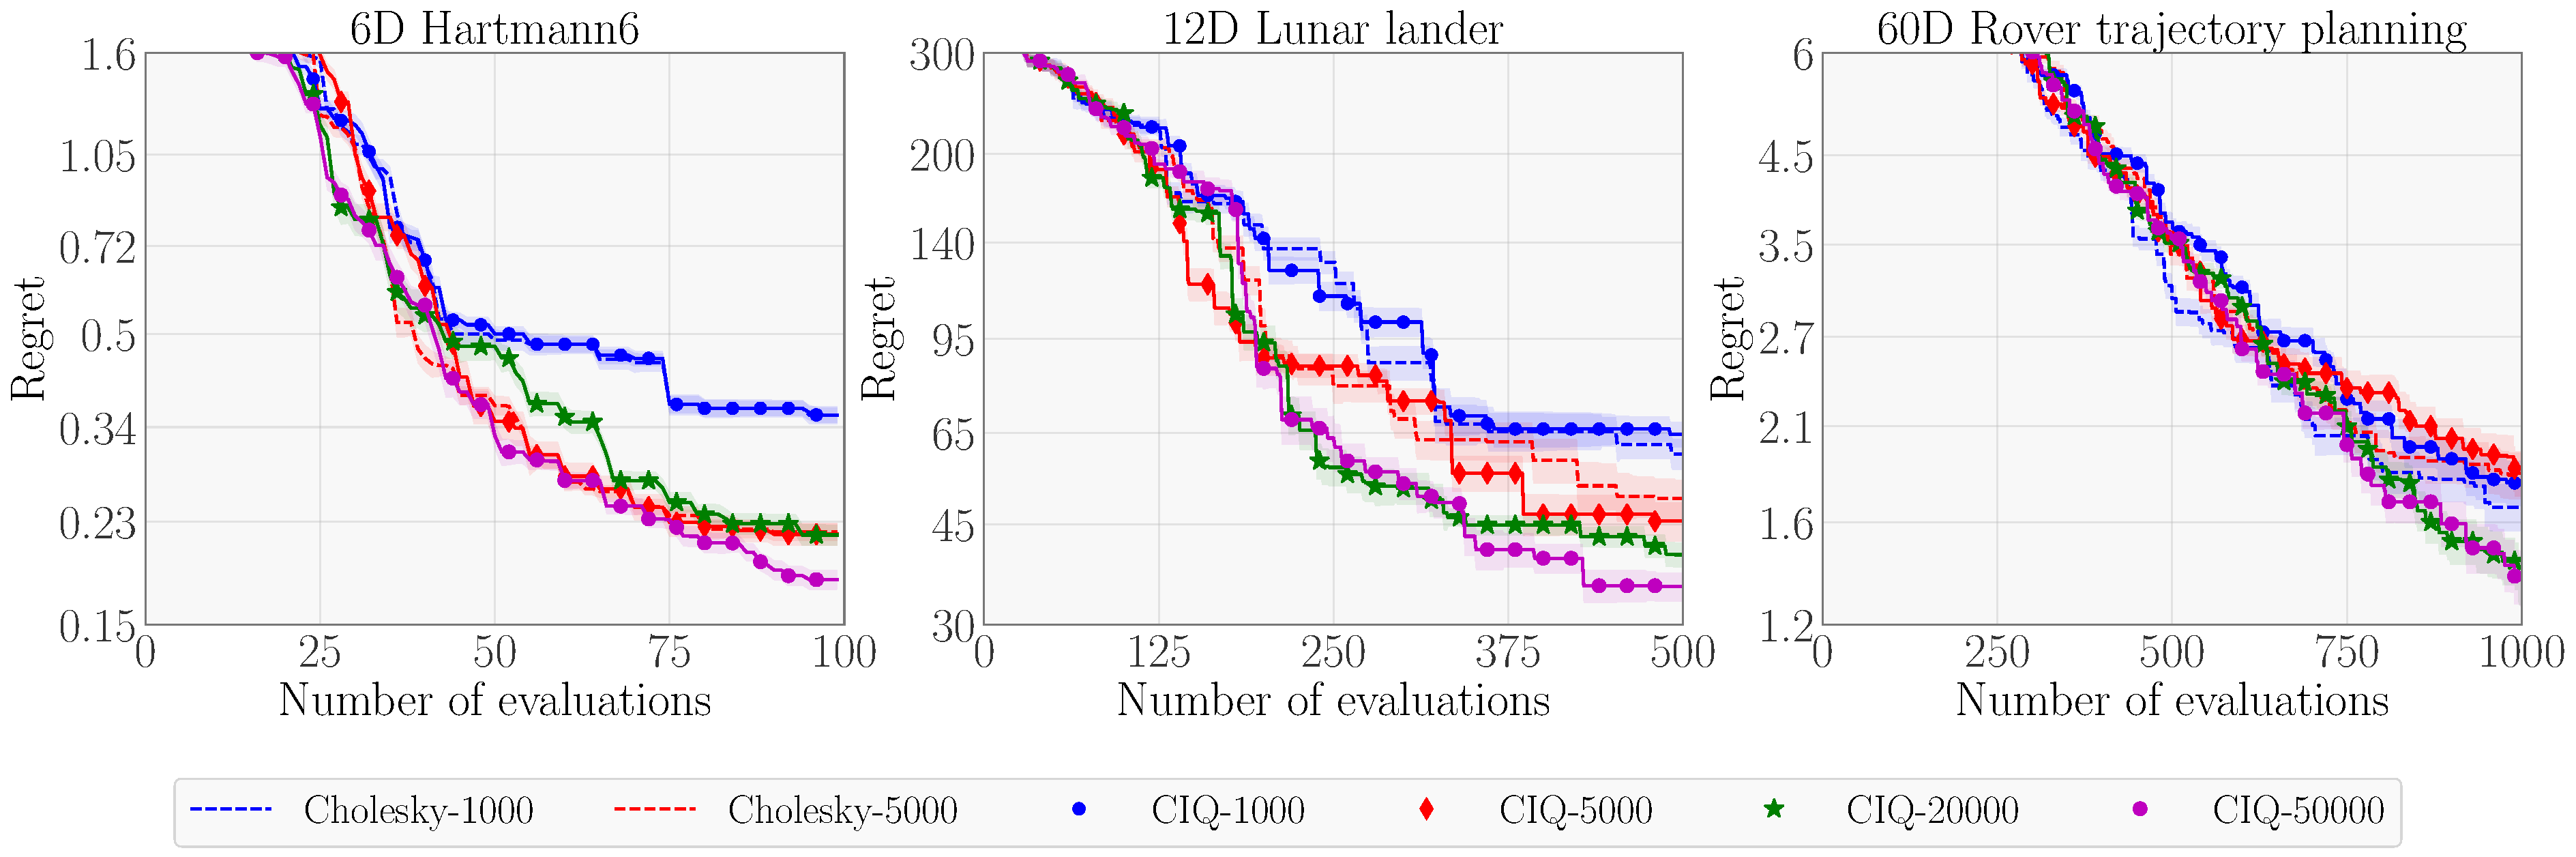
\includegraphics[width=0.97\linewidth]{figures/bo_ciq.pdf}
  \caption[
    A comparison of sampling methods for Bayesian optimzation (BayesOpt) via Thompson sampling.
    BayesOpt is applied to the Hartmann ($D=6$) and Lunar Lander ($D=12$) functions.
  ]{
    A comparison of sampling methods for Bayesian optimzation (BayesOpt) via Thompson sampling.
    BayesOpt is applied to the ({\bf left}) Hartmann ($D=6$), ({\bf middle}) Lunar Lander ($D=12$), and ({\bf right}) Rover ($D=60$) problems.
    Methods: TS-Chol-$\langle T \rangle$ draws posterior samples with Cholesky at $T$ candidate points.
    TS-CIQ-$\langle T \rangle$ draws posterior samples with CIQ.
    Larger $T$ results in better optimization.
    CIQ enables scaling to $T\geq50,\!000$.
  }
  \label{fig:bayesopt}
\end{figure}

We perform Bayesian optimization on three high-dimensional black-box functions: a classical test function ({\bf Hartmann}, $D=6$) and two robotics simulations ({\bf Lunar Lander}, $D=12$; {\bf Rover}, $D=60$).
For each problem we use exact Gaussian processes (no approximations) as the surrogate model and Thompson sampling as the acquisition function.
Our goal is to determine whether CIQ sampling is beneficial by allowing us to scale to larger candidate set sizes.

\paragraph{Baselines.}
With sufficient quadrature points and msMINRES iterations, we can reduce the error of CIQ to machine precision (see \cref{thm:ciq_convergence}). Therefore,
we limit the baseline methods to exact sampling methods, and do not consider stochastic approximations \cite{rahimi2008random} or methods that rely on inducing points \cite{wilson2020efficiently}.
We measure the performance of Thompson sampling as a function of the candidate set size $T$.
We run Thompson sampling Bayesian optimization with $T=1,\!000$, $T=5,\!000$, $T=20,\!000$, and $T=50,\!000$.
We use Cholesky ({\bf TS-Chol}) for $T=1,\!000$ and $T=5,\!000$, and we use CIQ ({\bf TS-CIQ}) for $T=20,\!000$ and $T=50,\!000$.
Note that it would be very challenging and impractical to use Cholesky with $T\geq10,\!000$, both due to its quadratic memory and its cubic time complexity.

\paragraph{Optimization performance.}
We plot the log regret of the Thompson sampling variants in \cref{fig:bayesopt}.
From these figures we can make several observations.
By increasing $T=1,\!000$ to $T=50,\!000$, the final log regret is significantly lowered on all problems.
We re-iterate that $T=50,\!000$ is largely impractical with Cholesky sampling methods.
Large candidate sets have previously only been possible with approximate sampling methods.
